\pdfminorversion=4
\documentclass[aspectratio=169]{beamer}

\mode<presentation>
{
  \usetheme{default}
  \usecolortheme{default}
  \usefonttheme{default}
  \setbeamertemplate{navigation symbols}{}
  \setbeamertemplate{caption}[numbered]
  \setbeamertemplate{footline}[frame number]  % or "page number"
  \setbeamercolor{frametitle}{fg=white}
  \setbeamercolor{footline}{fg=black}
} 

\usepackage[english]{babel}
\usepackage[utf8x]{inputenc}
\usepackage{tikz}
\usepackage{courier}
\usepackage{array}
\usepackage{bold-extra}
\usepackage{minted}
\usepackage[thicklines]{cancel}
\usepackage{fancyvrb}

\xdefinecolor{dianablue}{rgb}{0.18,0.24,0.31}
\xdefinecolor{darkblue}{rgb}{0.1,0.1,0.7}
\xdefinecolor{darkgreen}{rgb}{0,0.5,0}
\xdefinecolor{darkgrey}{rgb}{0.35,0.35,0.35}
\xdefinecolor{darkorange}{rgb}{0.8,0.5,0}
\xdefinecolor{darkred}{rgb}{0.7,0,0}
\definecolor{darkgreen}{rgb}{0,0.6,0}
\definecolor{mauve}{rgb}{0.58,0,0.82}

\title[2019-10-17-pyhep-awkward]{Awkward 1.0}
\author{Jim Pivarski}
\institute{Princeton University -- IRIS-HEP}
\date{October 17, 2019}

\usetikzlibrary{shapes.callouts}

\begin{document}

\logo{\pgfputat{\pgfxy(0.11, 7.4)}{\pgfbox[right,base]{\tikz{\filldraw[fill=dianablue, draw=none] (0 cm, 0 cm) rectangle (50 cm, 1 cm);}\mbox{\hspace{-8 cm}
\includegraphics[height=1 cm]{princeton-logo-long.png}\hspace{0.1 cm}\raisebox{0.1 cm}{
\includegraphics[height=0.8 cm]{iris-hep-logo-long.png}}\hspace{0.1 cm}}}}}

\begin{frame}
  \titlepage
\end{frame}

\logo{\pgfputat{\pgfxy(0.11, 7.4)}{\pgfbox[right,base]{\tikz{\filldraw[fill=dianablue, draw=none] (0 cm, 0 cm) rectangle (50 cm, 1 cm);}\mbox{\hspace{-8 cm}
\includegraphics[height=1 cm]{princeton-logo.png}\hspace{0.1 cm}\raisebox{0.1 cm}{
\includegraphics[height=0.8 cm]{iris-hep-logo.png}}\hspace{0.1 cm}}}}}

% Uncomment these lines for an automatically generated outline.
%\begin{frame}{Outline}
%  \tableofcontents
%\end{frame}

% START START START START START START START START START START START START START

\begin{frame}{asdf}
adsf
\end{frame}

\begin{frame}[fragile]{Layer 2: pybind11 of C++}
\vspace{0.5 cm}
\hfill\mbox{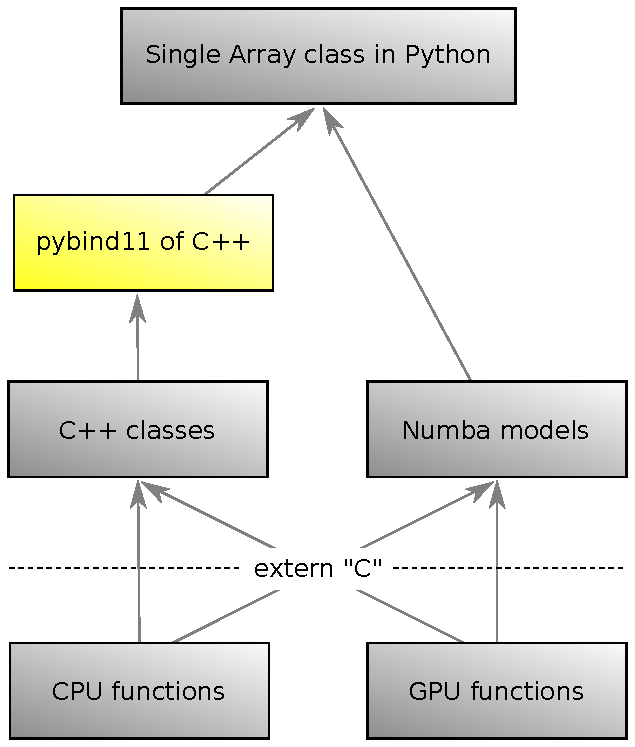
\includegraphics[height=4 cm]{awkward-1-0-layers-mini-pybind11.pdf}\hspace{-0.75 cm}}

\scriptsize
\vspace{-4.45 cm}
\begin{columns}
\column{1.1\linewidth}
\begin{minted}{python}
import awkward1, numpy

content = awkward1.layout.NumpyArray(numpy.arange(10)*1.1)
listA   = awkward1.layout.ListOffsetArray32(
            awkward1.layout.Index32(numpy.array([0, 3, 3, 5, 6, 10])),
            content)
listB   = awkward1.layout.ListOffsetArray32(
            awkward1.layout.Index32(numpy.array([0, 3, 4, 4, 5])),
            listA)

print(awkward1.tolist(listA))
\end{minted}

\vspace{-0.5 cm}
\begin{verbatim}
[[0.0, 1.1, 2.2], [], [3.3, 4.4], [5.5], [6.6, 7.7, 8.8, 9.9]]
\end{verbatim}
\begin{minted}{python}
print(awkward1.tolist(listB))
\end{minted}

\vspace{-0.5 cm}
\begin{verbatim}
[[[0.0, 1.1, 2.2], [], [3.3, 4.4]], [[5.5]], [], [[6.6, 7.7, 8.8, 9.9]]]
\end{verbatim}
\begin{minted}{python}
print(awkward1.tolist(listB[:, ::-1, ::2]))
\end{minted}

\vspace{-0.5 cm}
\begin{verbatim}
[[[3.3], [], [0.0, 2.2]], [[5.5]], [], [[6.6, 8.8]]]    (old awkward-array can't do this)
\end{verbatim}
\begin{minted}{python}
print(awkward1.tolist(listB[[0, 0, -1, -1], [0, -1, 0, -1], 1:-1]))
\end{minted}

\vspace{-0.5 cm}
\begin{verbatim}
[[1.1], [], [7.7, 8.8], [7.7, 8.8]]                     (mixing fancy and basic indexing)
\end{verbatim}
\end{columns}
\end{frame}

\begin{frame}{Layer 3: C++ classes}
\hfill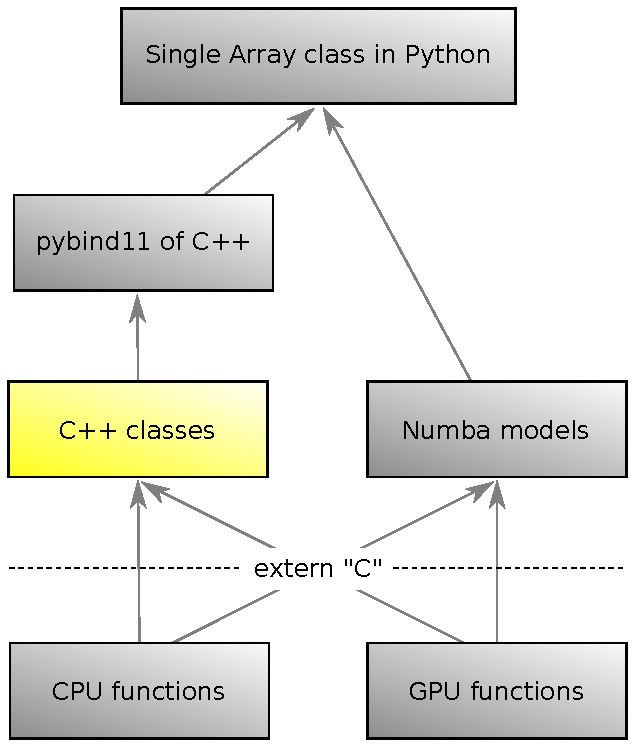
\includegraphics[height=4 cm]{awkward-1-0-layers-mini-cpp.pdf}

\vspace{-4 cm}
Stuff here
\end{frame}

\begin{frame}{Layer 3: Numba models}
\hfill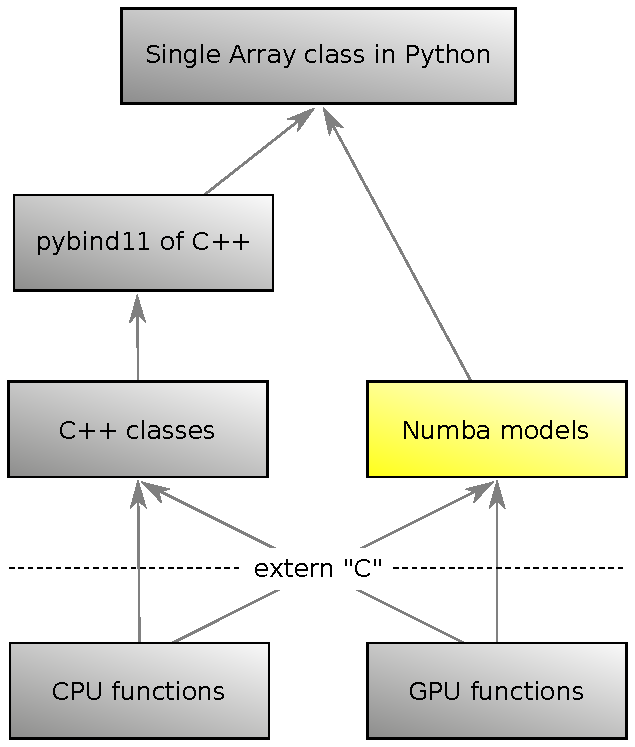
\includegraphics[height=4 cm]{awkward-1-0-layers-mini-numba.pdf}

\vspace{-4 cm}
Stuff here
\end{frame}

\begin{frame}{Layer 4: CPU functions}
\hfill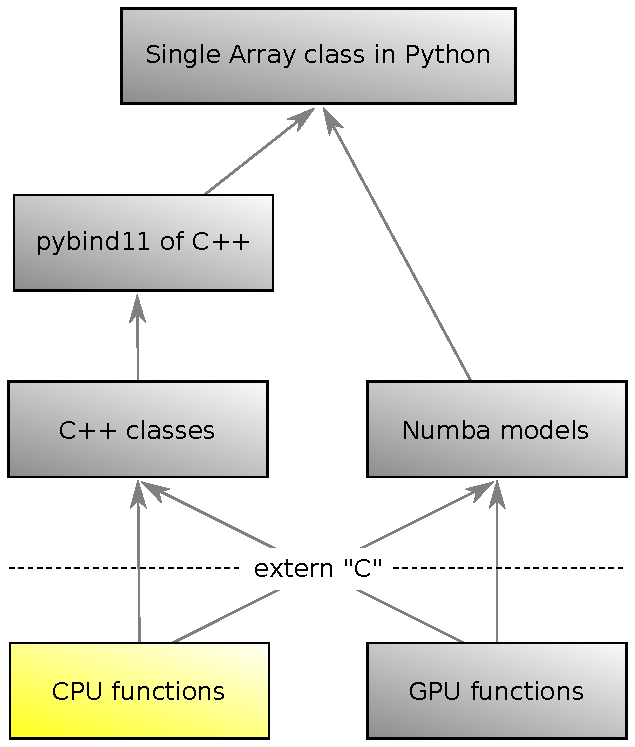
\includegraphics[height=4 cm]{awkward-1-0-layers-mini-cpu.pdf}

\vspace{-4 cm}
Stuff here
\end{frame}






\end{document}
